\paragraph{Monai VAE}\mbox{}
\subparagraph{Configuration}\mbox{}\\
\begin{table}[h!]
\centering
\begin{tabular}{|l|l|}
\hline
\textbf{Parameter} & \textbf{Value} \\
\hline
\multicolumn{2}{|c|}{\textbf{Training}} \\
\hline
Batch Size & 5 \\
\hline
Seed & 42 \\
\hline
Epochs & 1500 \\
\hline
Training Ratio & 0.9 \\
\hline
Number of Nodes & 1 \\
\hline
Device & CUDA \\
\hline
\multicolumn{2}{|c|}{\textbf{Model}} \\
\hline
Learning Rate & 0.0002 \\
\hline
Scan Shape & [1, 128, 128, 32] \\
\hline
Beta1 & 0.5 \\
\hline
Beta2 & 0.999 \\
\hline
Adversarial Weight & 0.01 \\
\hline
Perceptual Weight & 0.005 \\
\hline
KL Weight & 1e-5 \\
\hline
Fake 3D Ratio & 0.2 \\
\hline
Autoencoder Warm-Up Epochs & 5 \\
\hline
\multicolumn{2}{|c|}{\textbf{Dataset}} \\
\hline
Caching & Disk \\
\hline
Path & \url{/ravana/d3d\_work/micorl/data/ct\_images\_prostate\_32fixed/} \\
\hline
Image Size & 128 \\
\hline
Number of Slices & 32 \\
\hline
Window Width & 400 \\
\hline
Window Level & 60 \\
\hline
\end{tabular}
\caption{Configuration of the MONAI Autoencoder.}
\label{table:monai_autoencoder_params}
\end{table}

\newpage
\subparagraph{Training}\mbox{}\\

The model was trained for 1500 epochs. During the training, the loss was steadily decreasing. However, the generator loss started to increase after approximately 500 epochs. On the other hand, the loss of the generator during the validation phase did not show the same pattern.

\begin{figure}[H]
\minipage{0.49\textwidth}
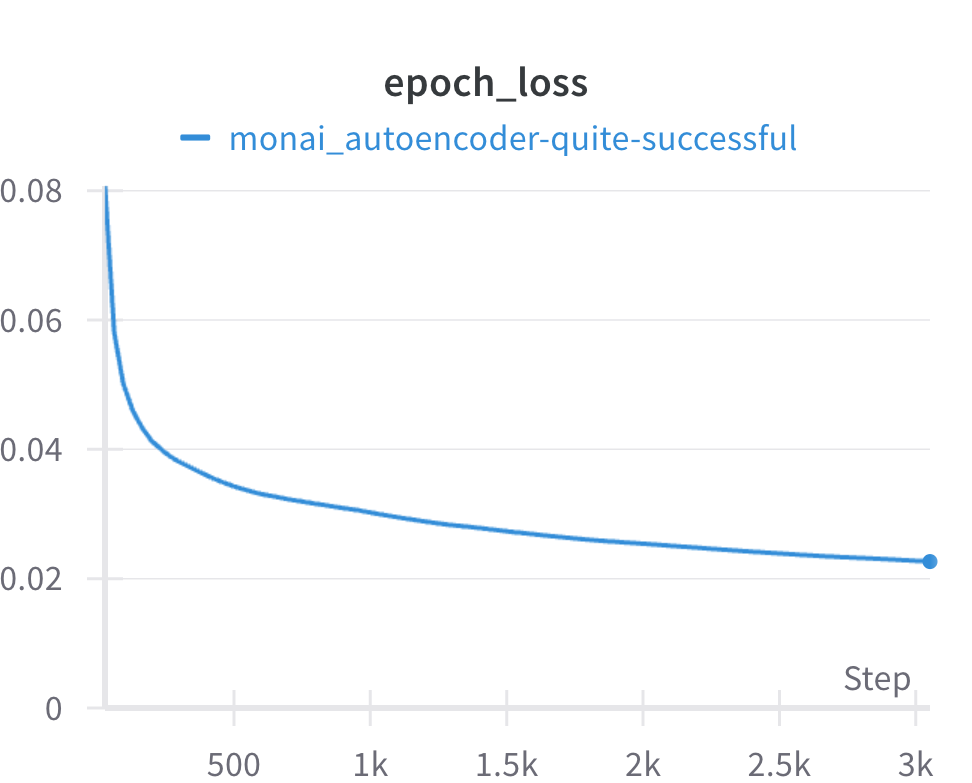
\includegraphics[width=\linewidth]{detailed_engineering/Monai Autoencoder/charts/epoch_loss.png}
\caption{Loss during the training.}
\endminipage\hfill
\minipage{0.49\textwidth}
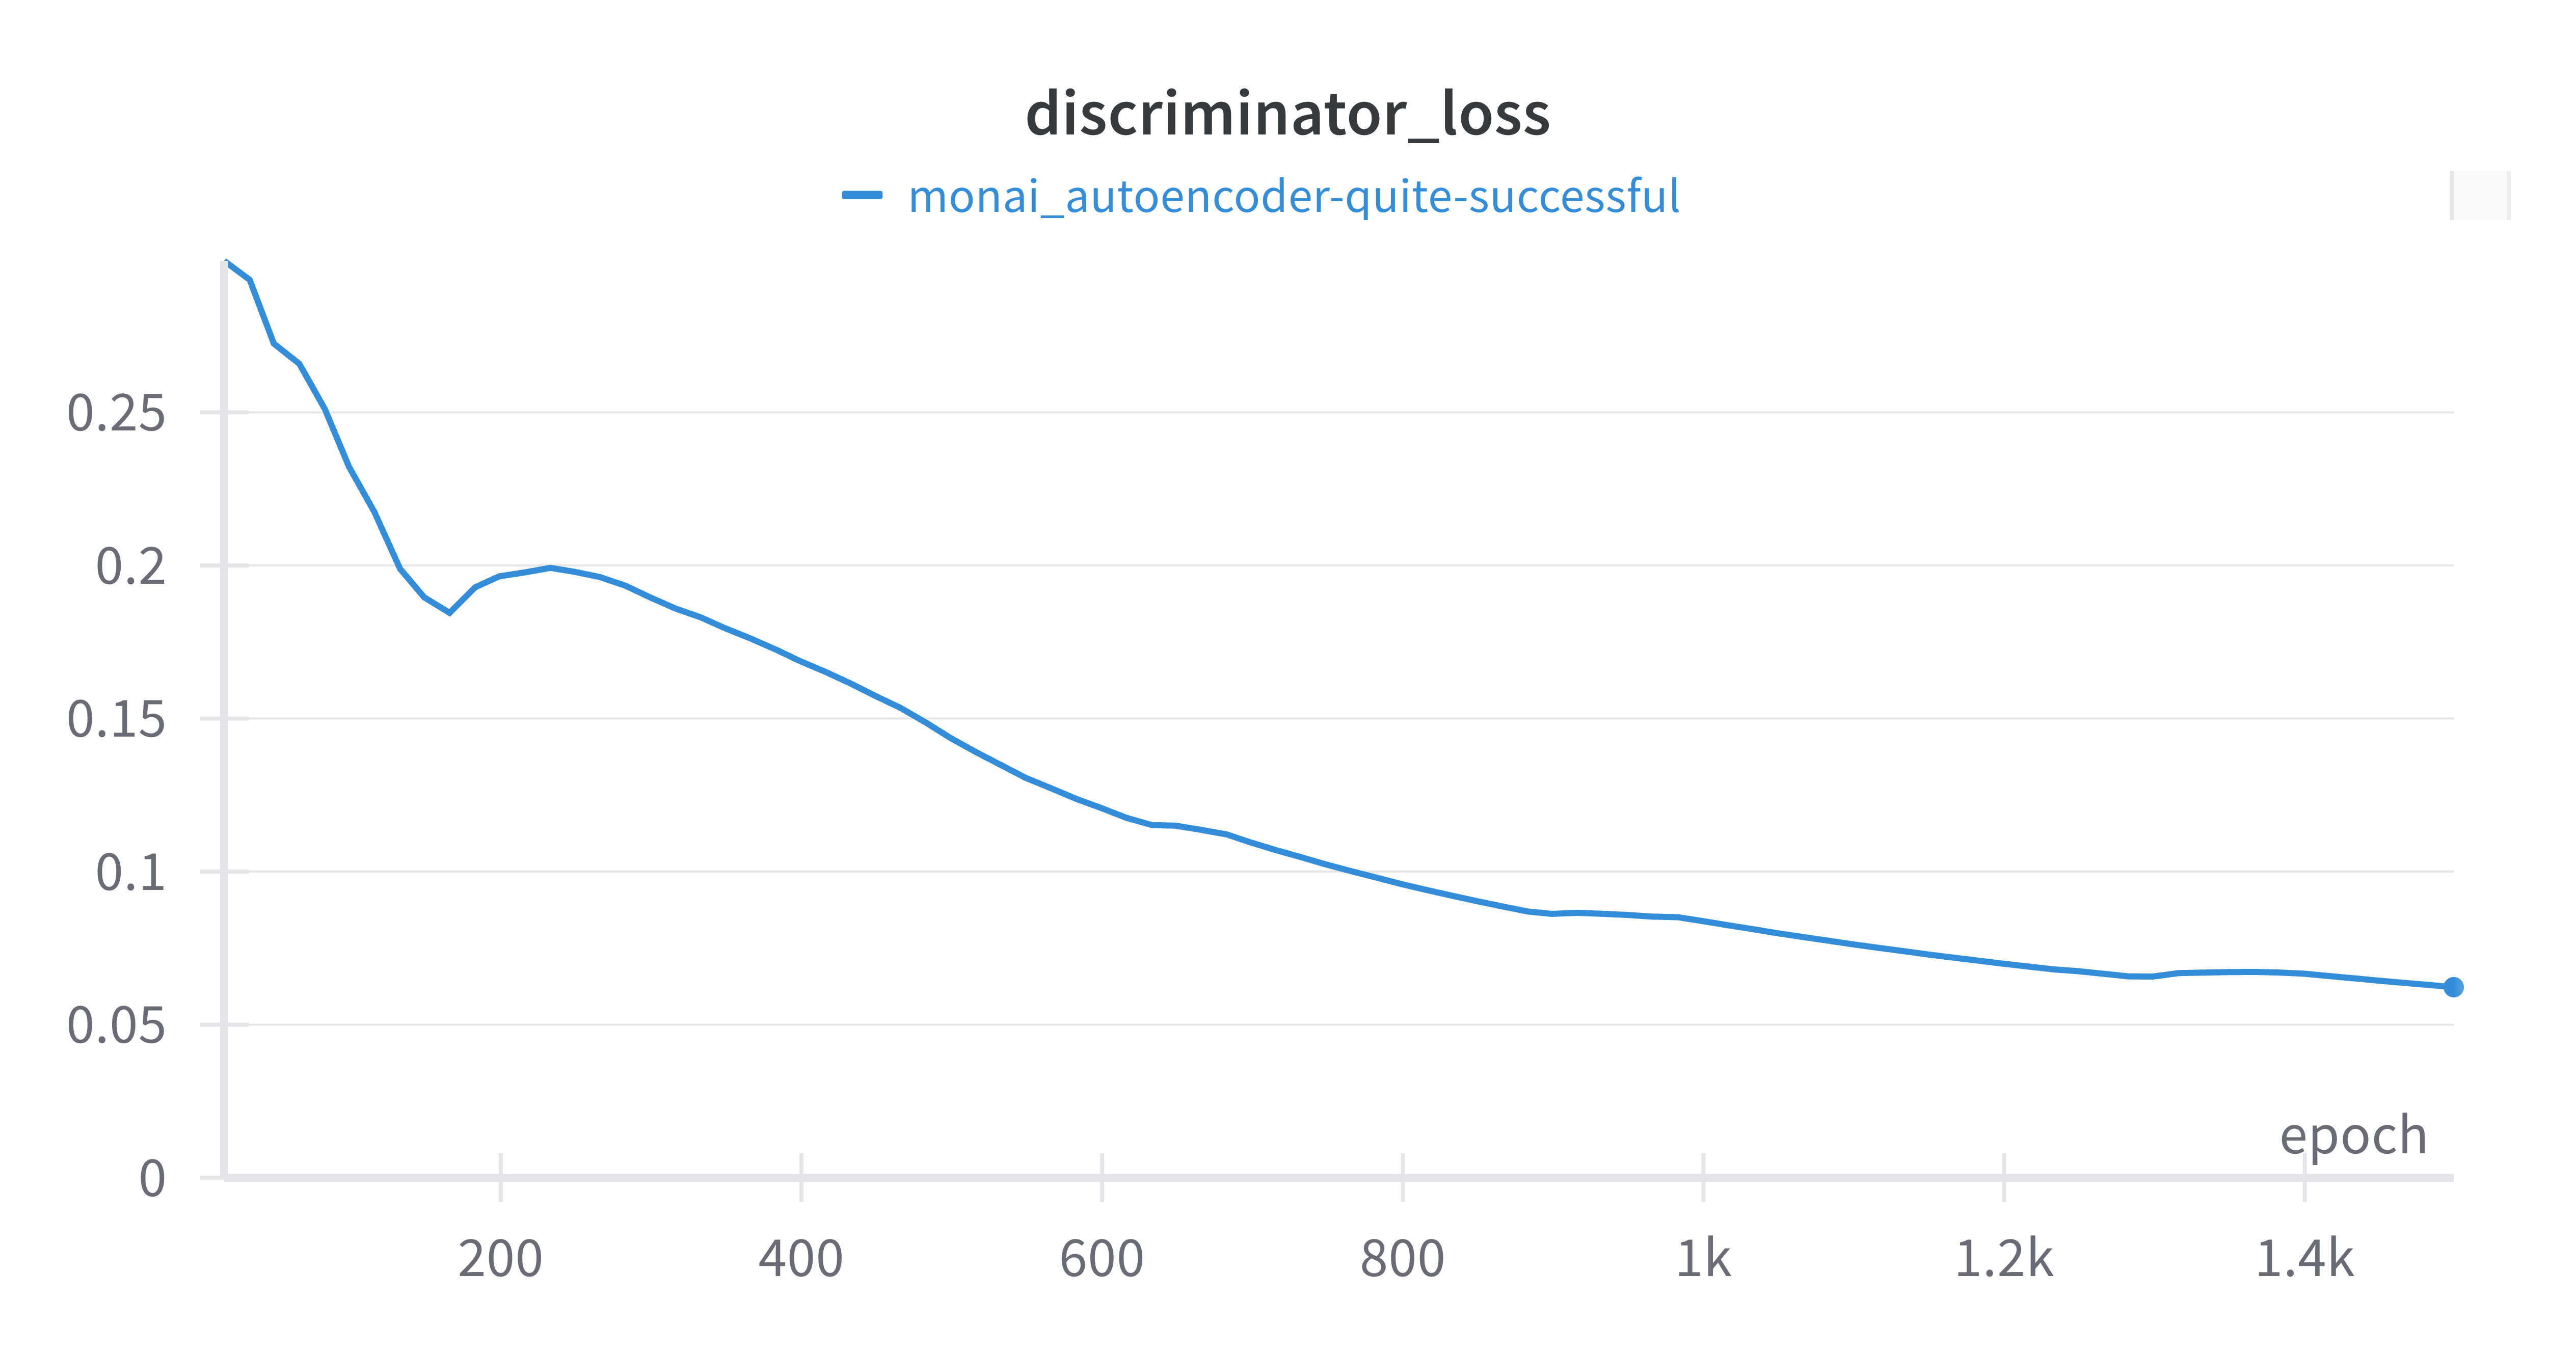
\includegraphics[width=\linewidth]{detailed_engineering/Monai Autoencoder/charts/discriminator_loss.png}
\caption{Discriminator loss during the training.}
\endminipage
\end{figure}

\begin{figure}[H]
\minipage{0.49\textwidth}
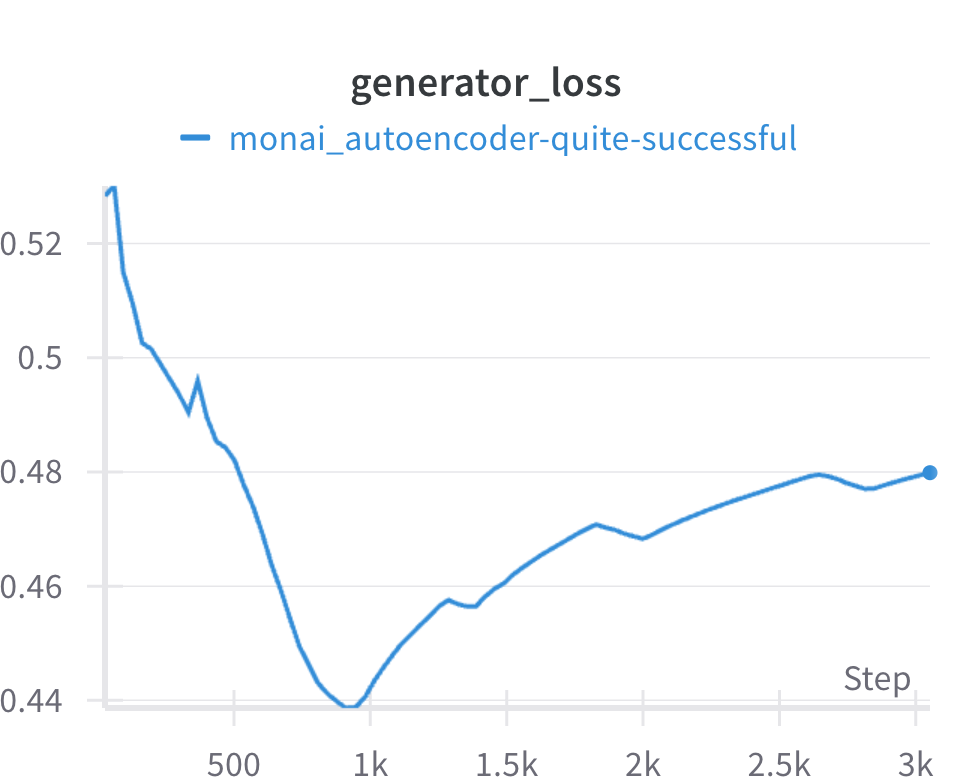
\includegraphics[width=\linewidth]{detailed_engineering/Monai Autoencoder/charts/generator_loss.png}
\caption{Generator loss during the training.}
\endminipage\hfill
\minipage{0.49\textwidth}
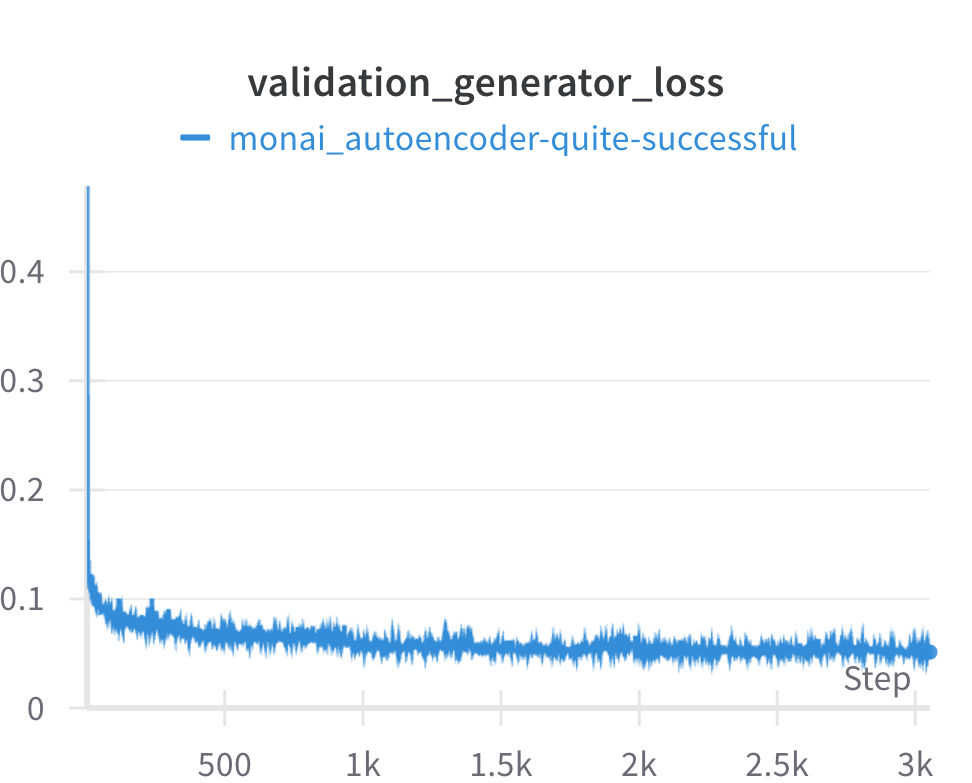
\includegraphics[width=\linewidth]{detailed_engineering/Monai Autoencoder/charts/val_generator_loss.png}
\caption{Generator loss during the validation.}
\endminipage
\end{figure}


\subparagraph{Results}\mbox{}\\

The resulting model was able to produce decent reconstructions. The difference between input and reconstruction was not large, as shown in Figure \ref{fig:monai-vae-comparison}. However, it may indicate that there is a field for improvement and the model parameters should be studied to see if the model is able to produce better reconstructions.

\begin{figure}[H]
    \centering
    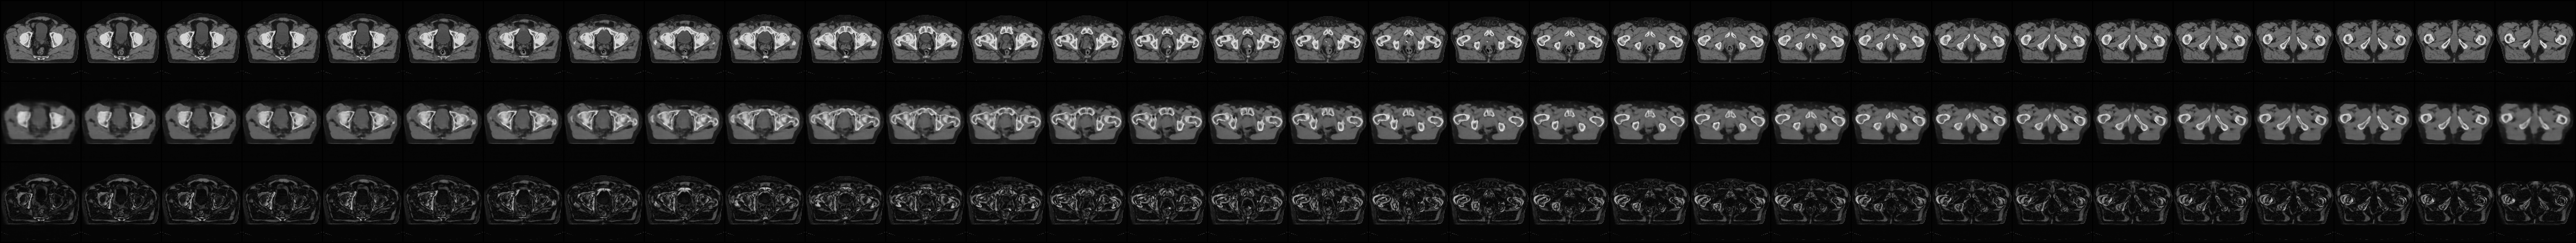
\includegraphics[width=\linewidth]{reports/monai_autoenc_comparison_full.png}
    \caption{Top - input, middle - reconstruction, bottom - difference.}
    \label{fig:monai-vae-comparison}
\end{figure}

